\chapter{Proposed Algorithm}\label{ch:algorithm} 
% Talk about what this chapter brings
The limitations identified by visual inspection of the data, the potential problems of the methods used by literature and the objective set for the algorithm as desribed in Chapter \ref{ch:design} are used in this chapter where a new algorithm is proposed able to detect deposition width and height. 

% Talk about the elements in this chapter.
First an overview is given of the steps in the new algorithm, followed by an in depth explanation of the methods used for each step. 

\section{Overview}
The common procedure in feature extraction from structured light is discussed in \ref{sc: previous_work}. The new algorithm is structured differently and this chapter is therefore divided into the following sections:

\subsection*{Image representation}
The images generated by the vision system are discussed in terms of data and the output as generated by the experimental setup is visualized.

\subsection*{Deposition Segmentation} 
The area where the deposition is present is detected and boundaries are determined. Template matching and a Triangle based algorithm are used to improve robustness. This way the segment where the laser illuminates the print bed and the deposition segment are seperated.

\subsection*{Laser Line Segmentation} 
After segmentation of print bed and deposition the laser line on the print bed is segmented from the background. A new thresholding method is proposed which is able to clarify the laser line edge at the point of segmentation. 

\subsection*{Width Extraction}
The deposition width is then extracted using te same template matching and triangle based algorithm as before. A smaller area is used to allow for local width measurement of the deposition at the edge of the laser line. 

\subsection*{Height Extraction}
The laser line is segmented from background reflections on the deposition utilizing the same method as used for seperation of the laser line on the bed. The height is then determined by measuring the difference in pixels between the edge of the laser line on the bed and the edge on the deposition. 


\section{Image representation}
Each image $I$ is represented as a matrix with $R$ rows, $C$ columns and $L$ layers or channels:
\begin{equation}
I \in \mathbb{Z}^{RxCxL}
\end{equation}
Values within the image can be represented by the following values where the subscripts $r,c,l$ are used for access to a pixel value:
\begin{equation}
I_{rcl} \in S_0 
\end{equation}
where the pixel values lie within the set:
\begin{equation}
S_0 = \{ I_{rcl} \in  \mathbb{Z} \mid 0 \leq I_{rcl} \leq 255 \}
\end{equation}
Graphical represenations of the data generated by the vision system are shown in Figure \ref{fig: image_channels}. The combined channels are shown in the red-green-blue (RGB) colorspace. The other channels are represented in gray-scale where the value $255$ is white and $0$ is black. A difference in intensity between channels is visible as $I_{rc1}$ is much brighter than the others.
\begin{figure}[!ht]
\centering
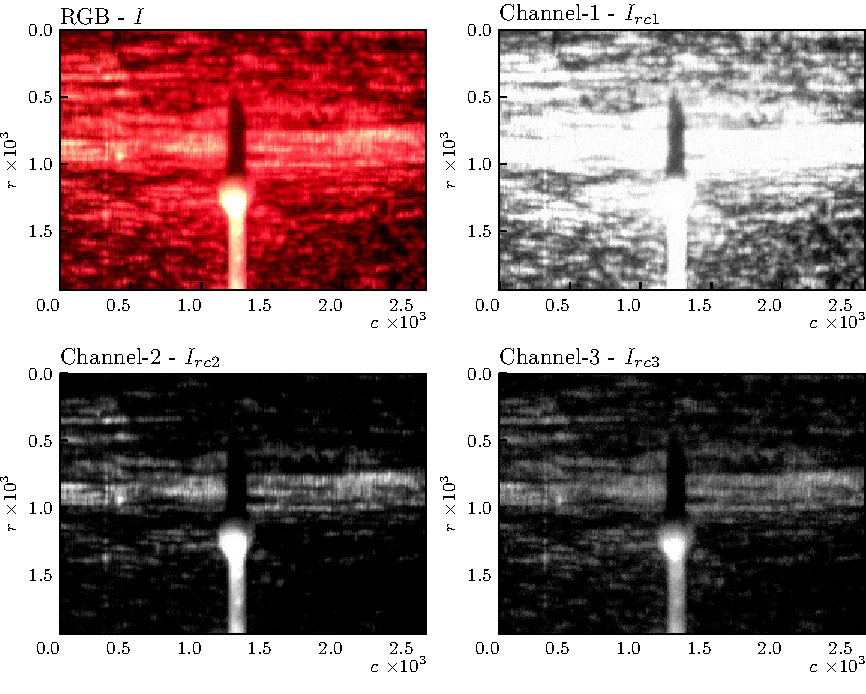
\includegraphics[width=\linewidth]{image_channels.pdf} 
\caption{Image channels in gray-scale and total image in RGB.}
\label{fig: image_channels}
\end{figure}


\section{Deposition Segmentation}
To segment the laser line from the background the depostion is seprated from the bed first. The algorithm used for segmentation of the laser line, as explained in Section \ref{sc: line segmentation}, would otherwise be disturbed.

\subsection*{Template matching} \label{ssc: template_matching}
% problem
Segmentation through intensity search is restrictive as explained in \ref{sc: line segmentation}. The sum of pixel values along an axis is the only measure used which ignores difference in distribution or pixel position. Although this approach works for segmentation of laser line and print bed this is not possible for deposition segmentation. Figure \ref{fig:profile} shows an ideal image of structured light by triangulation. The sum or distribution of the pixel values along the columns are the same. Position of pixel values is the only measure able to detect where the deposition is. 

% template matching
Template matching is therefore used which is able to detect difference in position and distribution. Segmenting the deposition from the bed is only posibble if the bed is visible in the image. The sides of the image therefore have to belong to the bed and can be used as a template. The template is defined as follows where the influence of noise is reduced by taking the mean of $\delta_1$ columns from the left and $C-\delta_2$ columns from the right side of the image $I$.
\begin{equation}
T_{rl} = \frac{1}{\delta_1+C-\delta_2}  \sum_{c \in S_2}  I_{rcl}, \quad \forall \, (r,l) \in S_1
\end{equation}
where
\begin{align}
S_1 &= \{(r,l)\in \mathbb {Z} \times \mathbb {Z} \mid 1 \leq r \leq R \land  1 \leq l \leq L \} \\
S_2 &= \{c \in \mathbb {Z} \mid 1 \leq c \leq \delta_1 \lor  \delta_2 \leq c \leq C \} 
\end{align} 
Two common methods for matching are cross-correlation and sum-of-squares. Normalized versions of these methods, as described in \cite{hisham2015template}, reduce influence of local intensity variations. Since it is assumed that the intensity of pixels on the bed are very similar to eachother and that pixels representing the deposition could be different, normalization is omitted. Furthermore, disturbances could make it impossible to differentiate between deposition and disturbance after normalization. Although both methods show good results the execution of the sum-of-squeres method is computational more efficient. The squared error at each pixel position is defined as:
\begin{equation}
SE_{rcl} = \left( I_{rcl} - T_{rl} \right)^2, \quad \forall \, (r,c,l) \in S_3
\end{equation}
where 
\begin{equation}
S_3 = \{(r,c,l)\in \mathbb {Z} \times \mathbb {Z} \times \mathbb {Z}  \mid 1 \leq r \leq R \land 1 \leq c \leq C \land 1 \leq l \leq L \} 
\end{equation}
and the sum-of-squared error for every columns is:
\begin{equation}
SSE_{cl} = \sum^{R}_{r=1} SE_{rcl} \quad \forall \, (c,l) \in S_4
\end{equation}
where
\begin{equation}
S_4 = \{(c,l)\in \mathbb {Z} \times \mathbb {Z} \mid 1 \leq c \leq C \land 1 \leq l \leq L \}  
\end{equation}
Figure \ref{fig: template_matching} shows the second channel $I_{rc2}$ of the image $I$ in gray-scale, the template $T_{r2}$, the squared errors $SE_{rc2}$ and the sum of squared errors $SSE_{c2}$ of an image generated by the vision system. A figure can be made for every channel of the image. The position of the large peak in $SSE_{c2}$ represents the deposition. $\delta_1$ and $C-\delta_2$ are both set to $130$ as an initial setting which in total is approximately $10\%$ of the total width $C=2592$.

\begin{figure}[!ht]
\centering
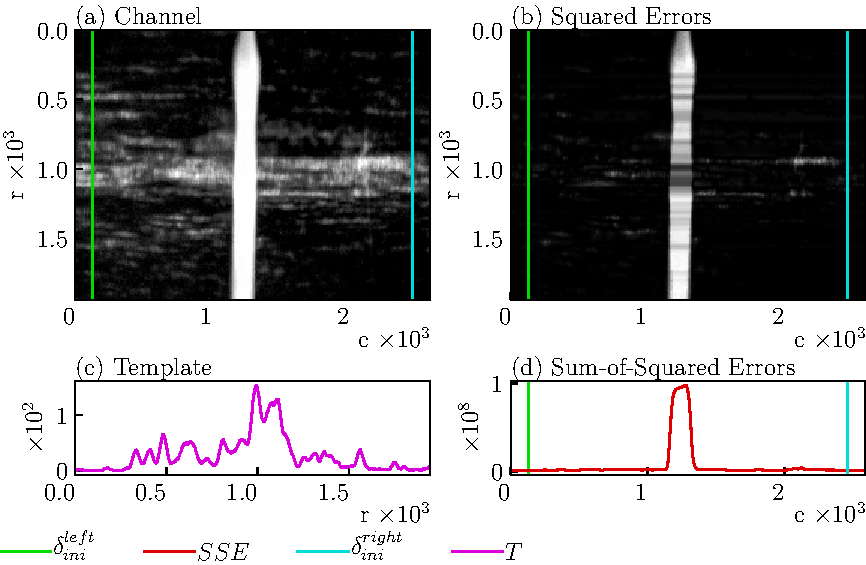
\includegraphics[width=\linewidth]{template_matching.pdf} 
\caption{Template Matching of $I_{rc2}$ with $\delta_1=C-\delta_2=130$.}
\label{fig: template_matching}
\end{figure}

\subsection*{Normalization} \label{ssc: normalization}
The sum of squared column errors for each layer are shown in Figure \ref{fig: normalized}b. Although the errors seam high for $SSE_{c1}$ they are relatively small compared to the errors of the columns used for calculation of the template. The sum of squared errors are in fact the variance of the column around the template. Before combining the errors of each layer into a total error they are normalized to unit variance. Each error is divided by the mean of the variance $M_l$ of the columns used for the template for each layer.
\begin{equation}
M_l = \frac{1}{\delta_1+\delta_2}  \sum_{c \in S_2}  SSE_{cl}, \quad \forall \, l \in S_5
\end{equation}
where
\begin{equation}
S_5 = \{l \in \mathbb {Z} \mid 1 \leq l \leq L \}  
\end{equation}
The normalized versions $NSSE_{cl}$ as shown in Figure \ref{fig: normalized}c of the errors then become:
\begin{equation}
NSSE_{cl} = \frac{SSE_{cl}}{M_l} \quad \forall \, (c,l) \in S_4
\end{equation}
The total error is then calculated as the euclidean distance between the layers as follows:
\begin{equation}
TE_{c} = \sqrt{ \sum_{l \in s_5} NSSE_{cl} } \quad \forall \, c \in S_6
\end{equation}
where 
\begin{equation}
S_6 = \{c \in \mathbb {Z} \mid 1 \leq c \leq C \}  
\end{equation}

\begin{figure}[!ht]
\centering
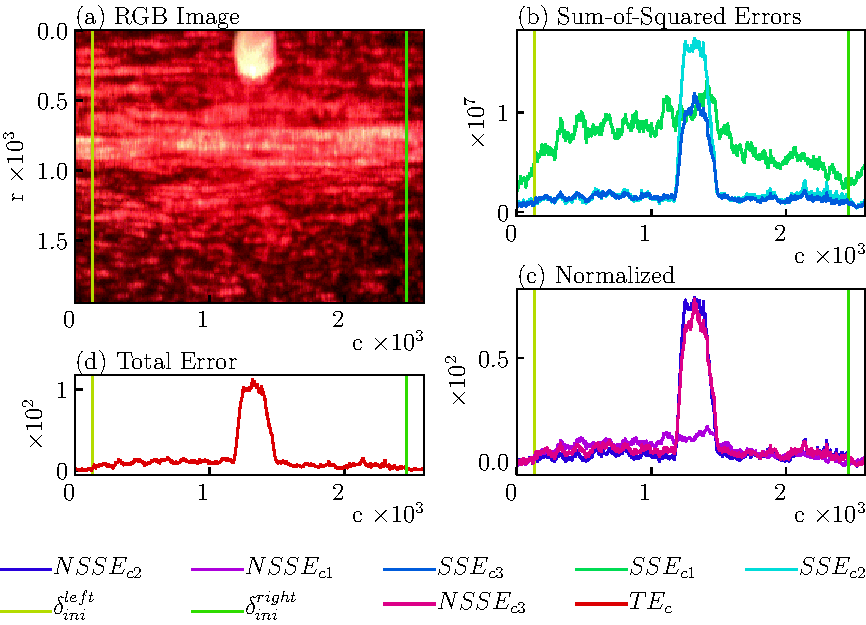
\includegraphics[width=\linewidth]{normalized.pdf} 
\caption{Total Error as euclidean distance of normalized sum-of-squared errors.}
\label{fig: normalized}
\end{figure}

\subsection*{Segmentation}\label{sc: triangle}
The total error $TE_c$ is used to seperate the deposition from the print bed. Differencing the total error $TE_c - TE_{c-1} \quad \forall \, c \in S_6$ and calculating the maximum and mininum as the seperation points is error prone as shown in Figure \ref{fig: triangle}b. The signal-to-noise ratio is low and a filter should have been applied to filter the noise. This is however not preferred as discussed in Section \ref{sc: previous_work}. Furthermore, calculating the extrema of the differenced series results in finding the points where the total error changes the most. It does however not find the points where the deposition starts. Figure \ref{fig: triangle}a shows the image in RGB with $\delta^{DIFF}_1$ and $\delta^{DIFF}_2$ as the points of seperation. A small part of the deposition is much wider than the rest which the method based on differencing does not detect. 

The Triangle algorithm as described in \cite{zack1977automatic} is used as a global thresholding method. This method is adapted to serve as a better alternative to seperation based on differencing. The first step is to form the piecewise triangle function $T_c$ as follows. The result is shown in Figure \ref{fig: triangle}c.
\begin{equation}
T_c = \left.
  \begin{cases}
    TE^{MN}, & \forall \, c \in S_2\\
    \frac{c-\delta_1}{TE^{AMAX} - \delta_1} \left( TE^{MAX} - TE^{MN} \right),  & \forall \, c \in S_7\\
    \frac{\delta_2-c}{\delta_2-TE^{AMAX}} \left( TE^{MAX} - TE^{MN} \right),  & \forall \, c \in S_8\\
  \end{cases}
  \right.
\end{equation}
where
\begin{align}
S_7 &= \{c \in \mathbb {Z} \mid \delta_1 \leq c \leq TE^{AMAX} \}  \\
S_8 &= \{c \in \mathbb {Z} \mid TE^{AMAX} \leq c \leq \delta_2 \}  
\end{align}
and
\begin{align}
TE^{MN} &= \frac{1}{\delta_1+C-\delta_2}  \sum_{c \in S_2}  TE_{c} \\
TE^{MAX} &= \{TE_{c'} \mid TE_{c'} > TE_{c} \quad \forall\, c \in S_6 \} \\
TE^{AMAX} &= \{c \mid TE_{c} = TE^{MAX} \}
\end{align}
\begin{figure}[!ht]
\centering
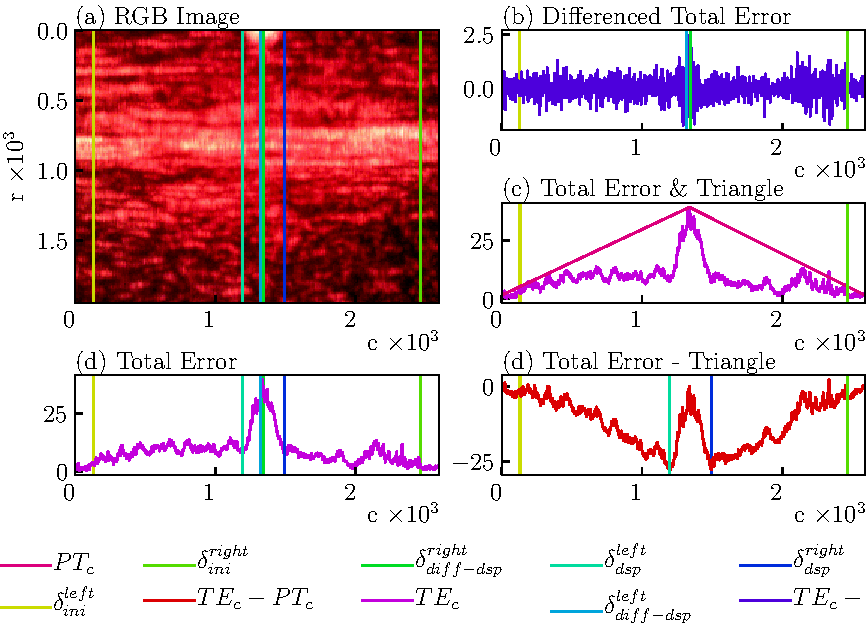
\includegraphics[width=\linewidth]{triangle.pdf} 
\caption{Triangle based segmentation versus differencing.}
\label{fig: triangle}
\end{figure}

\skippar
The points of seperation $\delta^{NEW}_1$ and $\delta^{NEW}_2$ are then found by calculating the minima of the difference as follows:
\begin{align}
\delta^{NEW}_1 &= \{c \mid D_c = D^{MIN}_1 \} \\
\delta^{NEW}_2 &= \{c \mid D_c = D^{MIN}_2 \} 
\end{align}
where 
\begin{align}
D_c &= TE_c - T_c \quad \forall \, c \in S_6 \\
D^{MIN}_1 &= \{D_{c'} \mid D_{c'} < D_{c} \quad \forall\, c \in S_7 \} \\
D^{MIN}_2 &= \{D_{c'} \mid D_{c'} < D_{c} \quad \forall\, c \in S_8 \} 
\end{align}
The results as shown in Figure \ref{fig: triangle}a show that the triangle based method is more sensitive to deposition change than the differencing based method. $\delta^{NEW}_1$ and $\delta^{NEW}_2$ completely seperate the deposition from the bed. The signal-to-noise ratio is very high which improves robustness. Furthermore, there are no parameters to be tuned as no filter is used. 


\section{Laser Line Edge Segmentation} \label{sc: line segmentation}

After segmentation of the deposition from the bed it is possible to segment the laser line from the bed. The line position serves as a reference point for height measurement. Furthermore, the width of the deposition is  determinant at the position of the laser. 

\subsection*{Thresholding}
Laser line position is ussually determant by detecting the peak gray-scale intensity value of each column. There are however data implied problems as described in Section \ref{sc: data limitations}. Saturation of pixels makes peak detection unreliable and inhomogenity in the line makes column wise detections hard. Width measurement of the line and taking the middle of the line as a reference point is of no use since the width of the laser line onto the bed might be different. 

Therefore a single edge is used as reference point and the mean of the row pixels is used as the intensity value. Using the image in gray-scale instead of all layers relies on the assumption that the laser line brightness is highest in the center of the line and is lower the further away from the middle. The image in gray-scale is shown in Figure \ref{fig: thresholding}a and is calculated by:
\begin{equation}
I^{gray}_{rc} = 0.299 I_{rc1} + 0.587 I_{rc2} + 0.114 I_{rc3}, \quad \forall \, (r,c) \in S_9
\end{equation}
where:
\begin{equation}
S_9 = \{(r,c)\in \mathbb {Z} \times \mathbb {Z} \mid 1 \leq r \leq R \land 1 \leq c \leq C \} 
\end{equation}
The mean of the pixels in each row not belonging to the deposition is shown in Figure \ref{fig: thresholding}b and is given by:
\begin{equation}
M_{r0} =  \frac{1}{\delta^{NEW}_1 + R - \delta^{NEW}_2}  \sum_{c \in S_{10}}  I^{gray}_{rc}, \quad \forall \, r \in S_{11}
\end{equation}
where:
\begin{align}
S_{10} &= \{c \in \mathbb {Z} \mid 1 \leq c \leq \delta^{NEW}_1 \lor \delta^{NEW}_2 \leq c \leq C \} \\
S_{11} &= \{r \in \mathbb {Z} \mid 1 \leq r \leq R \}
\end{align}
\begin{figure}[!ht]
\centering
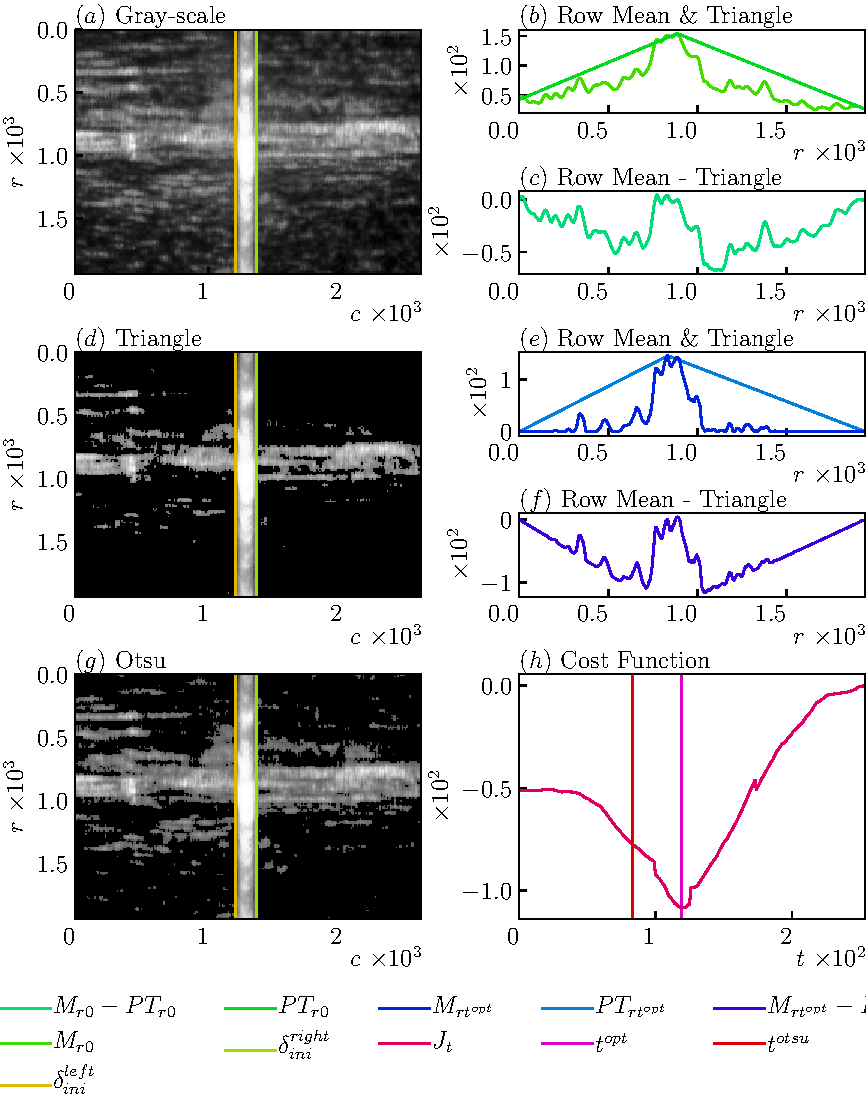
\includegraphics[width=\linewidth]{thresholding.pdf} 
\caption{Triangle based thresholding versus Otsu's method.}
\label{fig: thresholding}
\end{figure}
Using the Triangle algorithm as described in Section \ref{sc: triangle} to determine the segment where the edge is positioned is possible but very unreliable due to the amount of background noise in the image. Therefore thresholding is used to seperate background from foreground. Otsu's method as described in \cite{otsu1979threshold} is one the most used histogram based thresholding methods and the result of this method is shown in Figure\ref{fig: thresholding}g. Although it does a reseanable job seperating the background from the foreground the algorithm is not focused at clarifying the edge. 

A new thresholding method based upon the triangle algorithm is therefore proposed. This algorithm maximizes the distance between the maximum value of the row mean and the value at the position determant by the triangle algorithm as the edge. The optimal threshold value is found by:

\begin{equation}
t_{optimal} = \argmin_t J_t, \quad \forall \, t \in S_0
\end{equation}
where $J_t$ is the cost function given by:
\begin{equation}
J_t = \min_r D_{rt}, \quad \forall \, r \in S_{12}
\end{equation}
with:
\begin{equation}
S_{12} = \{ r \in \mathbb {Z} \mid 1 \leq r \leq \argmax_r M_{rt}  \}
\end{equation}
where $D_{rt}$ is defined as the difference between the mean row intensity $M_{rt}$ at a certain threshold $t$ and $T_{rt}$ is the triangle calculated as before in Section \ref{sc: triangle}. The upper edge of the laser line is chosen as reference point. Therefore the cost function is focused at minimizing $D_{rt}$ for all rows before the place where the maximum row intensity $\argmax_r M_{rt}$ occurs.
\begin{equation}
D_{rt} = M_{rt} - T_{rt}
\end{equation}
The mean row intensity $M_{rt}$ is given by:
\begin{equation}
M_{rt} =  \frac{1}{\delta^{NEW}_1 + C - \delta^{NEW}_2}  \sum_{c \in S_{10}}  I^{gray}_{rc}, \quad \forall \, (r,I^{gray}_{rc},t) \in S_{13}
\end{equation}
where:
\begin{equation}
S_{13} = \{ (r,I^{gray}_{rc},t) \in \mathbb {Z} \times \mathbb {Z} \times \mathbb {Z} \mid 1 \leq r \leq R \land I^{gray}_{rc} \geq t \land 0 \leq t \leq 255 \}
\end{equation}
The cost function $J_t$ at every threshold value is calculated and is displayed in Figure \ref{fig: thresholding}h. The threshold $t^{otsu}$ is the value as determined by Otsu's method and is clearly sub-optimal in maximizing the difference in mean row intensity between rows at the edge. The optimal threshold as determined by the new algorithm is shown as $t^{optimal}$. The row mean $M_{rt_{optimal}}$ and triangle $T_{rt_{optimal}}$ created for this threshold are shown in Figure \ref{fig: thresholding}ef and the thresholded image $I^{gray} > t_{optimal}$ is shown in Figure \ref{fig: thresholding}d. 

\subsection*{Segmentation}
After thresholding, the rows containing the edge are segmented. Figure \ref{fig: edge_segmentation} shows the image in RGB and Gray-scale with the section containing the edge as the rows between $\delta_3$ and $\delta_4$ which are defined as:
\begin{align}
\delta_3 &= \argmin_r D_{rt}, \quad \forall \, r \in S_{12} \\
\delta_4 &= \argmax_r M_{rt_{optimal}}, \quad \forall \, r \in S_{11}
\end{align}
\begin{figure}[!ht]
\centering
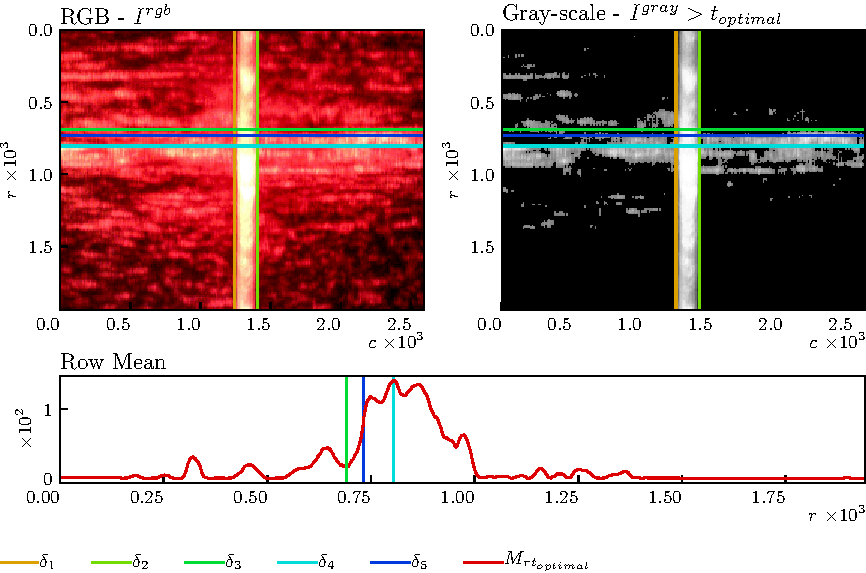
\includegraphics[width=\linewidth]{edge_segmentation.pdf} 
\caption{Edge segmentation of the laser line on the print bed.}
\label{fig: edge_segmentation}
\end{figure}
These rows will be used for width extraction. The row at which the edge actual is positioned is defined as the row $\delta_5$ at which the mean pixel value lies exactly in the middle of the mean pixel values of the rows $\delta_3$ and $\delta_4$. The peak value of the differenced series could also be used but is sensitive to noise and requires filtering which is not preferred. 
\begin{equation}
\delta_5 = \{r \mid M_{rt_{optimal}} = \left( M_{\delta_4t_{optimal}} - M_{\delta_3t_{optimal}} \right) / 2 \}
\end{equation}

\section{Width measurement}
The rows containing the laser line edge, $\delta_3 \leq r \leq \delta_4$, are used to determine the width of the deposition at the edge. A single row could be used for width determination depending on the amount of disturbance in the laser line. If there was a clear distinction between laser line and background then $\delta_3$ and $\delta_4$ would be closer to eachother. A perfect laser line without disturbance would result in $\delta_4 = \delta_3 +1$.

% template
The width is determant using the same template matching method as described in Subsection \ref{ssc: template_matching}. The columns used for forming the template are all columns $S_{10}$ belonging to the bed. The template is formed according to:

\begin{equation}
T_{rl} = \frac{1}{\delta^{NEW}_1+C-\delta^{NEW}_2}  \sum_{c \in S_{10}}  I_{rcl}, \quad \forall \, (r,l) \in S_1
\end{equation}

\skippar
The normalized errors for each layer and the total error are determant according to Subsection \ref{ssc: normalization}. The Triangle algorithm is applied to find the edges $\delta_7$ and $\delta_8$ of the deposition at the rows which include the laser line edge $\delta_5$. The result is shown in Figure \ref{fig: width_extraction}. The width $W$ of the deposition is then calculated by:

\begin{equation}
W = \delta_7-\delta_6
\end{equation}
\begin{figure}[!ht]
\centering
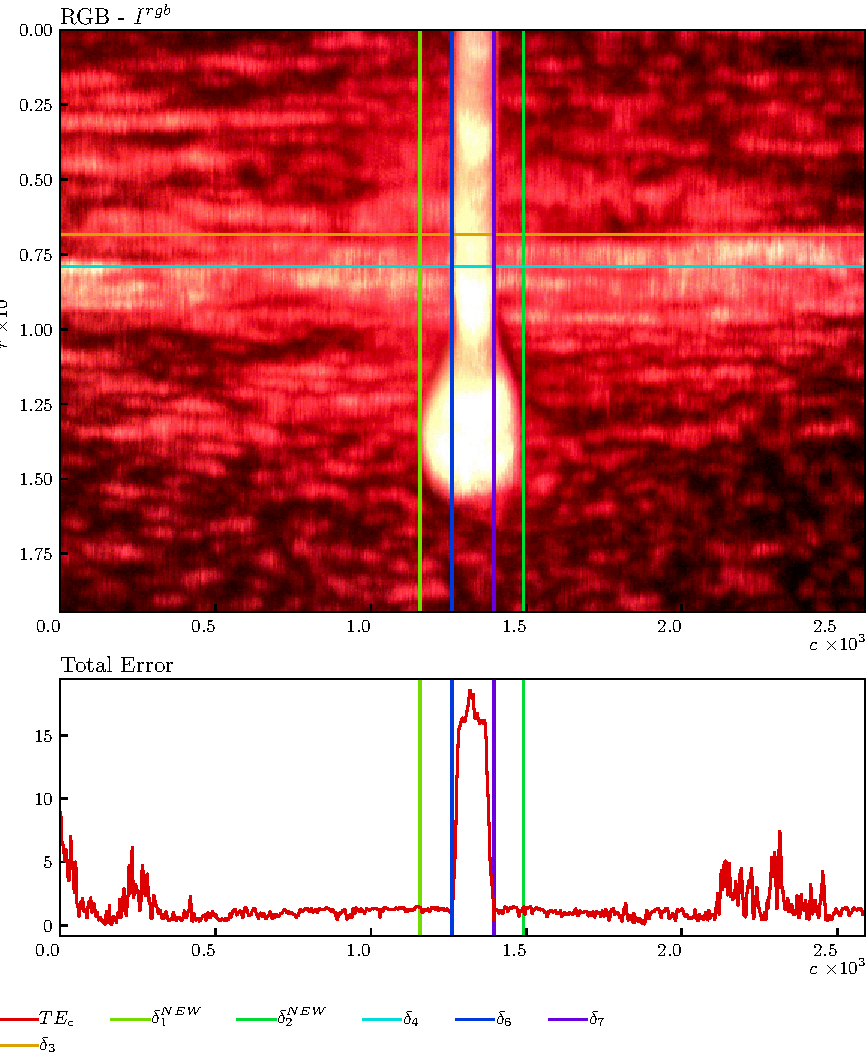
\includegraphics[width=\linewidth]{width_extraction.pdf} 
\caption{Width extraction at the position of the laser line edge.}
\label{fig: width_extraction}
\end{figure}

\section{Height measurement}
To measure deposition height $H$, the difference between the laser line edge on the bed $\delta_5$ and the edge on the deposition $\delta_{10}$ is calculated. The actual height can be calculated from the angle of the laser relative to the bed. 
\begin{equation}
H = \delta_{10}-\delta_5
\end{equation}
The results of all algorithms needed for height extraction are shown in Figure \ref{fig: height_extraction}. The bed, which are all columns $c$ in $S_{10}$, is globally thresholded with threshold $t^{BED}_{optimal}$ using the Triangle threshold method as described in Section \ref{sc: line segmentation}. The columns representing the deposition $\delta_6 \leq c \leq \delta_7$ are thresholded utilizing the same method with $t^{DEPOSITION}_{optimal}$ as a result. The row means after the application of these thresholds are displayed as $M^{BED}_{rt_{optimal}}$ for the bed and $M^{DEPOSITION}_{rt_{optimal}}$ for the deposition.
\begin{figure}[!ht]
\centering
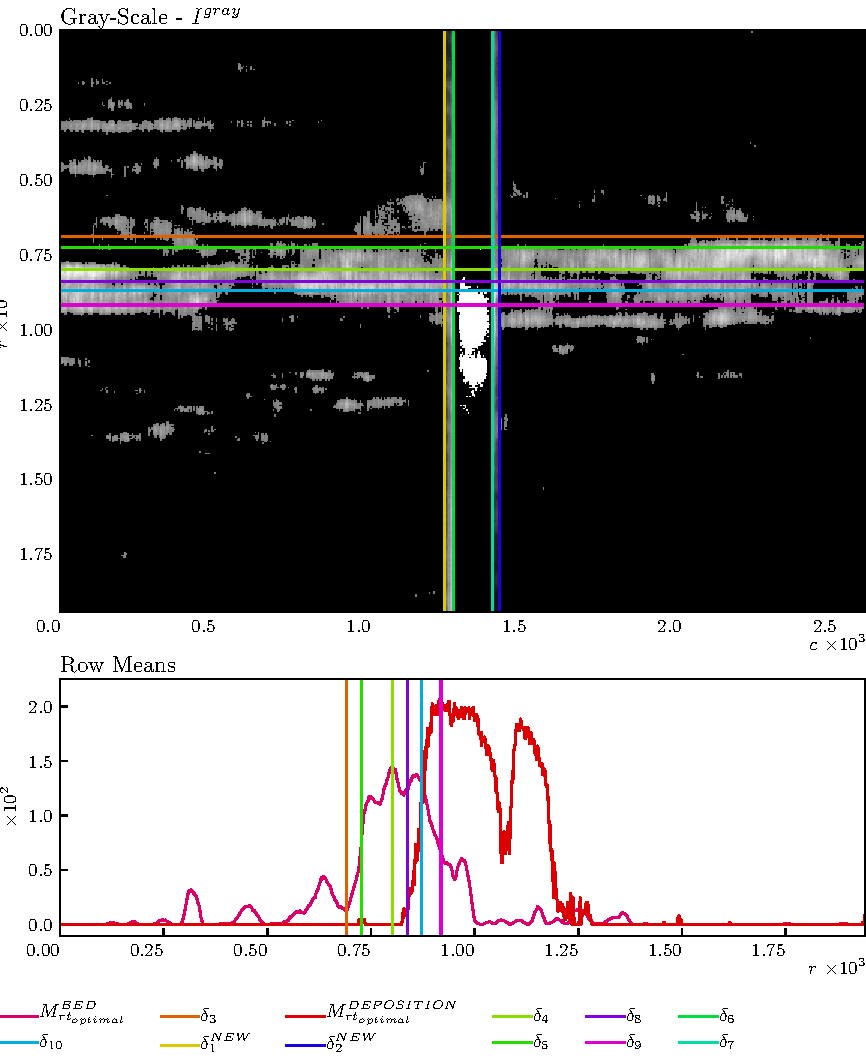
\includegraphics[width=\linewidth]{height_extraction.pdf} 
\caption{Height extraction.}
\label{fig: height_extraction}
\end{figure}



